\begin{figure}
	\centering
	\subfigure[Simulink shema za vodenje v notranjih koordinatah]
	{
		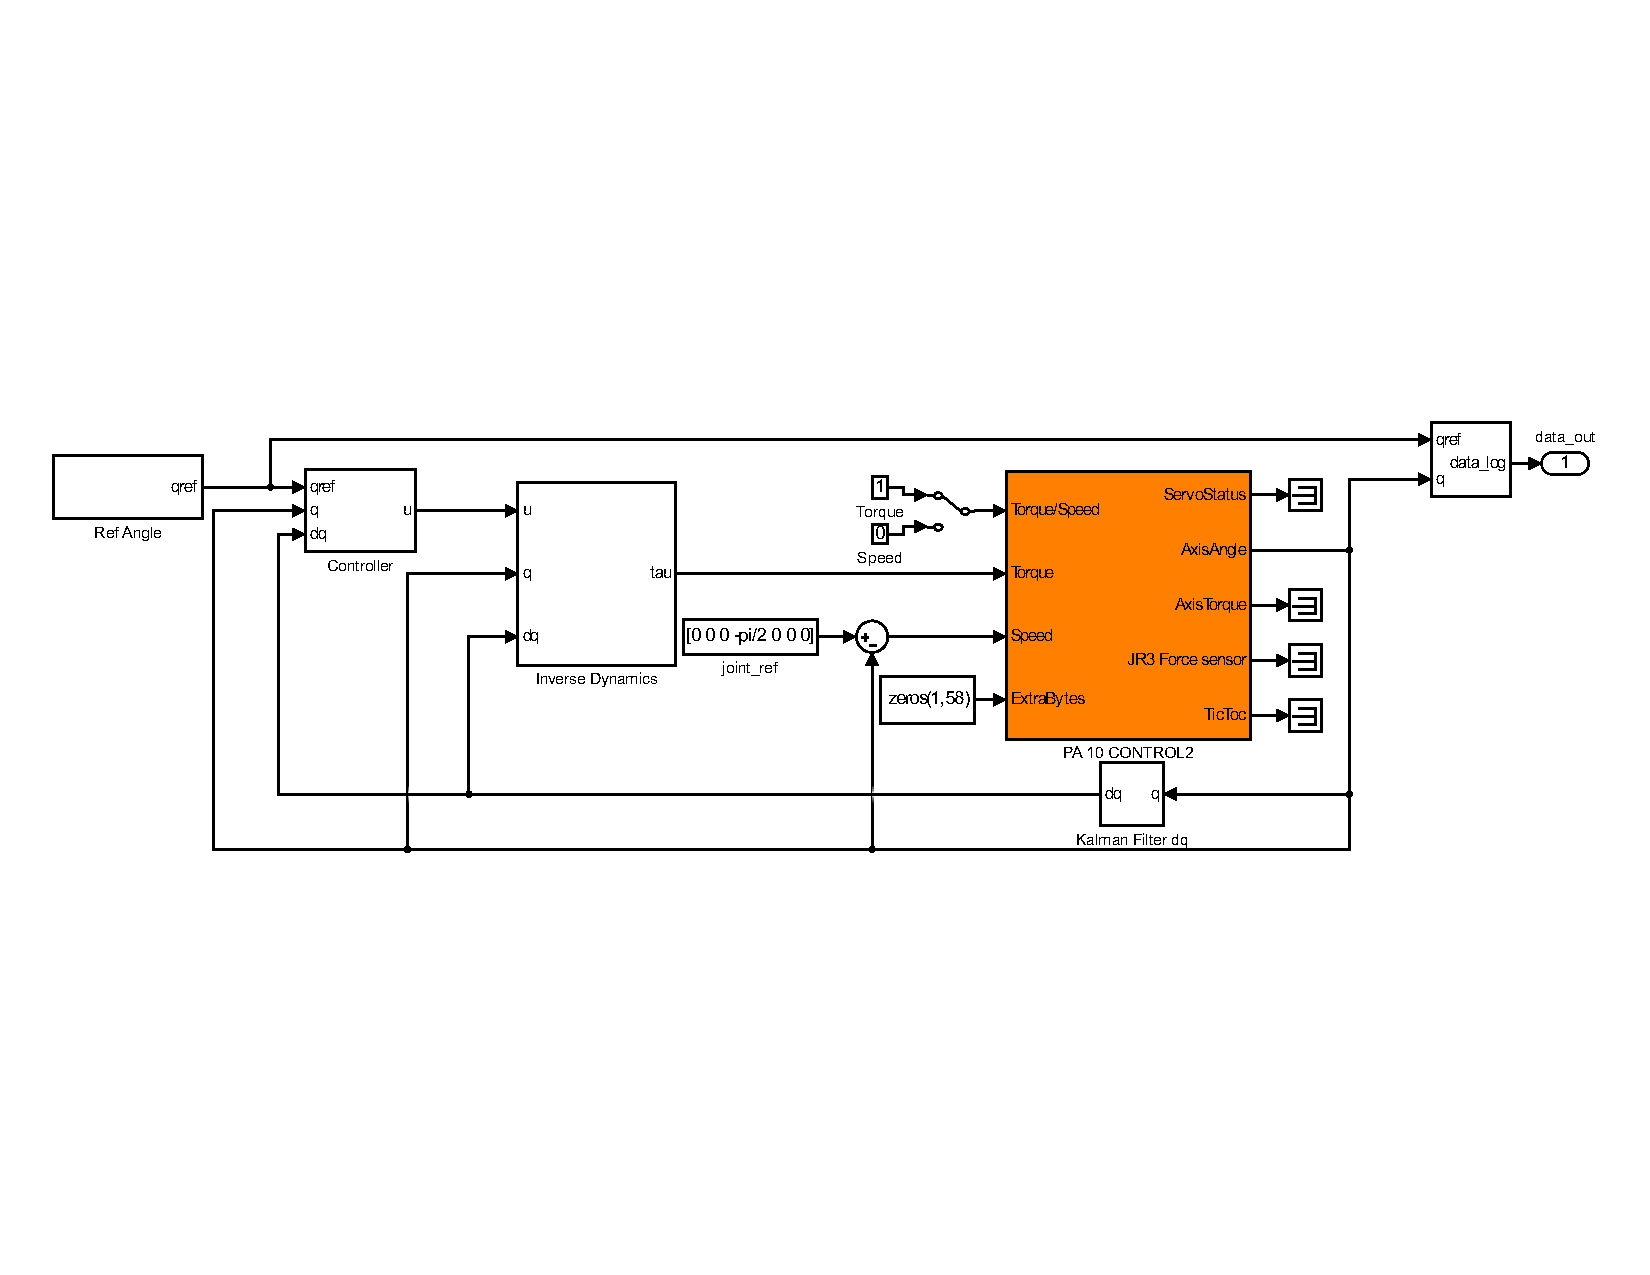
\includegraphics[trim={2cm 8cm 4cm 4cm},scale=0.35]{./Slike/notranje_koor_tq.pdf}
	}
	\subfigure[Simulink shema za vodenje v zunanjih koordinatah]
	{
		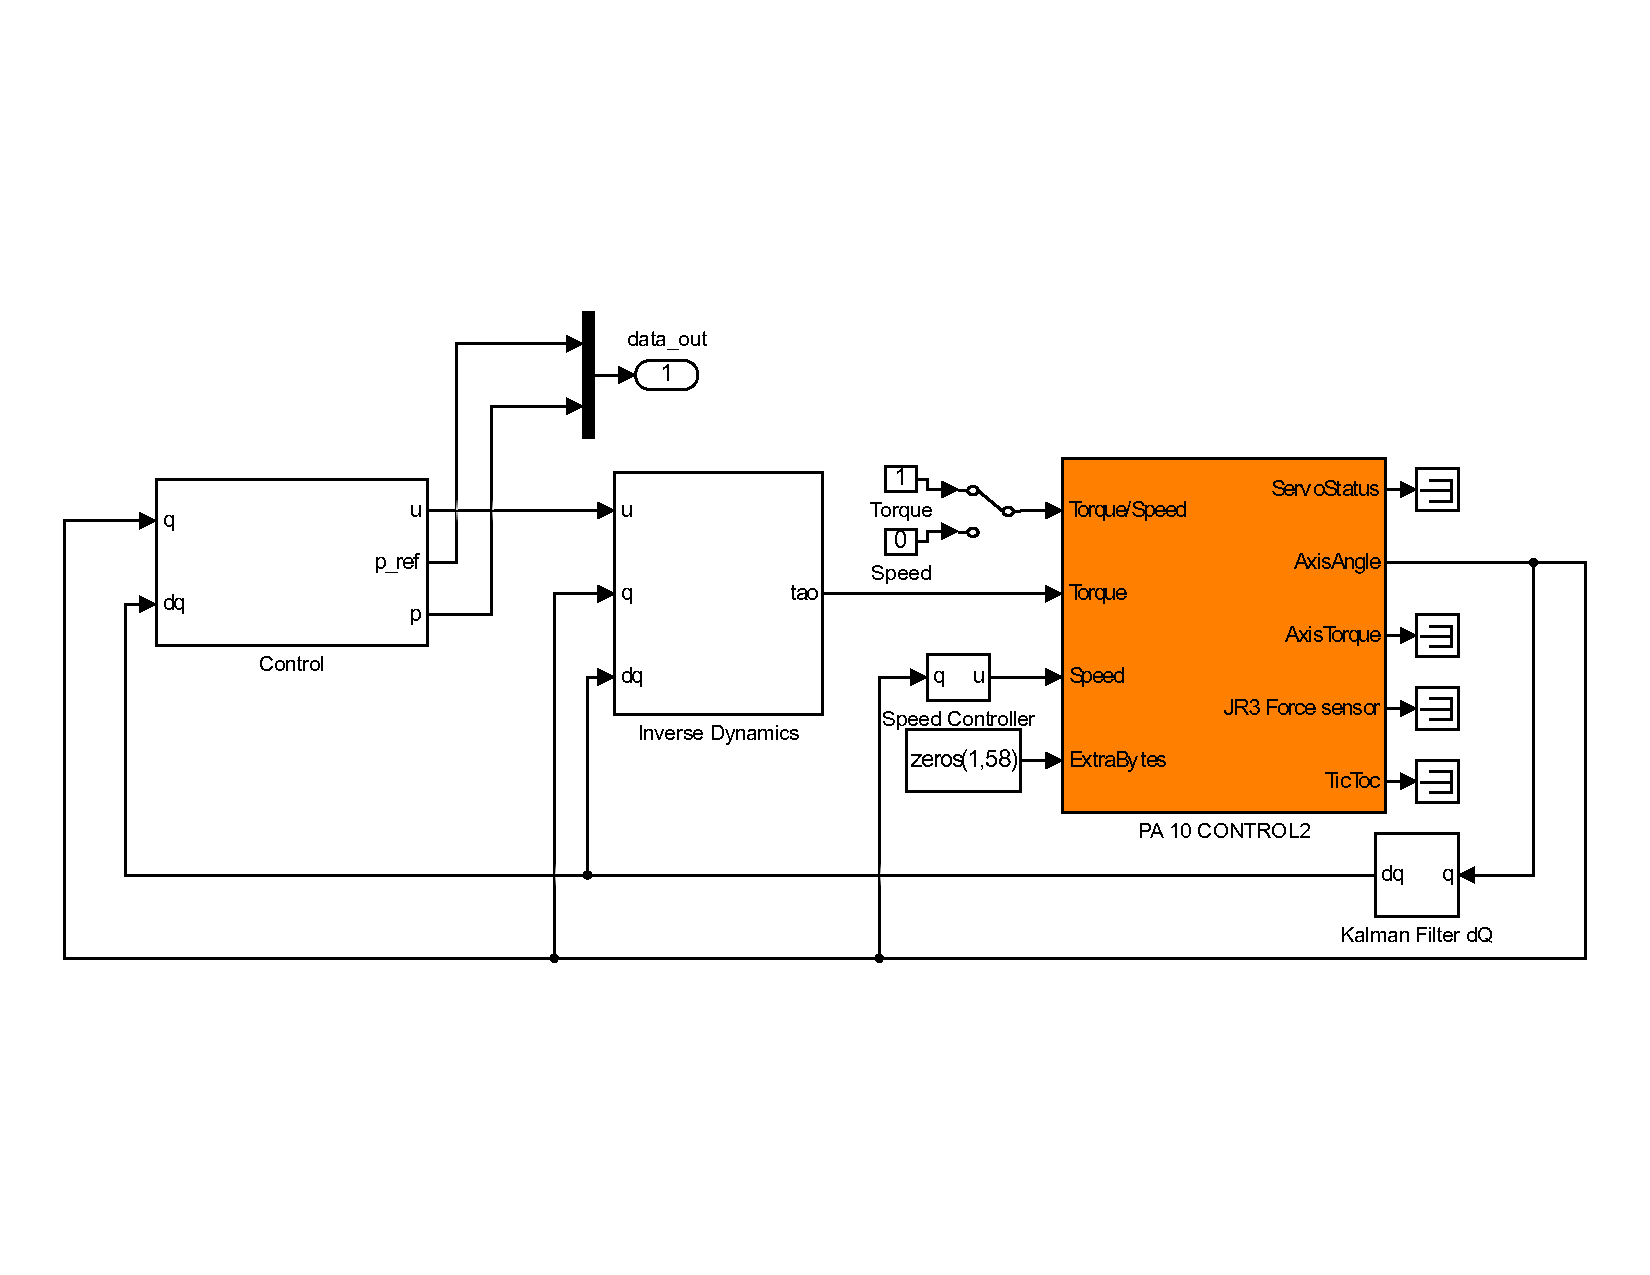
\includegraphics[trim={4cm 6cm 6cm 1.5cm},scale=0.35]{./Slike/zunanje_koor_tq.pdf}
	}
	\subfigure[Simulink shema za impedan\v{c}no vodenje]
	{
		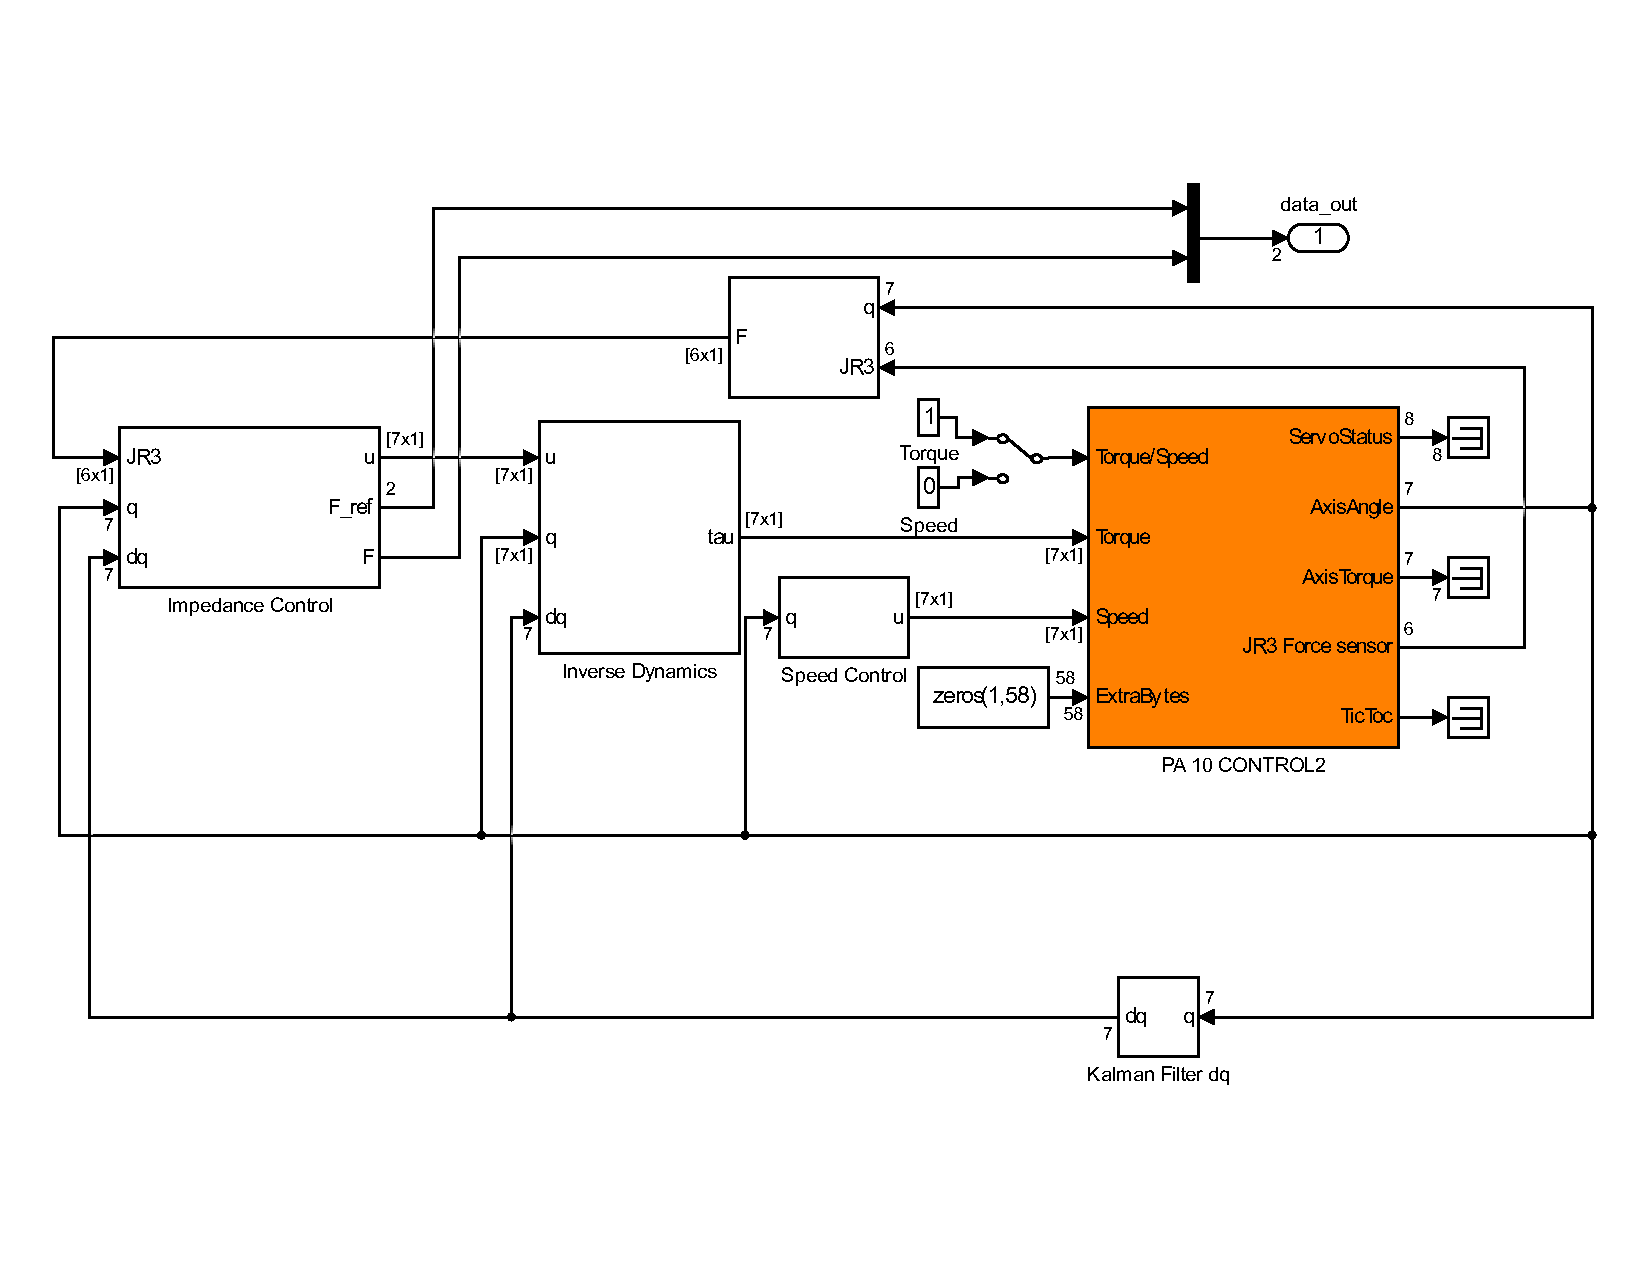
\includegraphics[trim={2cm 4cm 2cm 3cm},scale=0.35]{./Slike/impedance_control.pdf}
	}
	\caption{Simulink sheme za vodenje v navornem na\v{c}inu. V shemo je vklju\v{c}eno stikalo za preklapljanje med hitrostnim ter navornim na\v{c}inom. Hitrostno vodenje smo uporabili za pozicioniranje v izhodično lego poskusa.}
	\label{fig:simulink_tq_control}
\end{figure}
